\documentclass{article}

\usepackage{a4}
\usepackage{graphicx}

\begin{document}

\title{Modelos Determinísticos de Investigação Operacional - Trabalho 1\\
    \large\emph{MIEI - Universidade do Minho}}
\author{Sofia Santos - A89615 \and Ema Dias - A89518 \and
    Sara Queiróz - A89491 \and Tânia Teixeira - A89613}

\date{Ano Letivo 2020/21}    

\maketitle

\newpage

\section{Formulação}

Neste problema temos um drone que precisa de percorrer um conjunto de linhas elétricas de alta tensão à procura de alguma interferência. Queremos que o drone percorra a menor distância possível, mas que percorra todas as linhas pelo menos uma vez. Para além de viajar pelas linhas, em qualquer sentido, o drone também pode viajar pelo ar.

De acordo com o maior nº de estudante do nosso grupo, o nosso mapa de linhas é o seguinte:

\begin{figure}[h]
    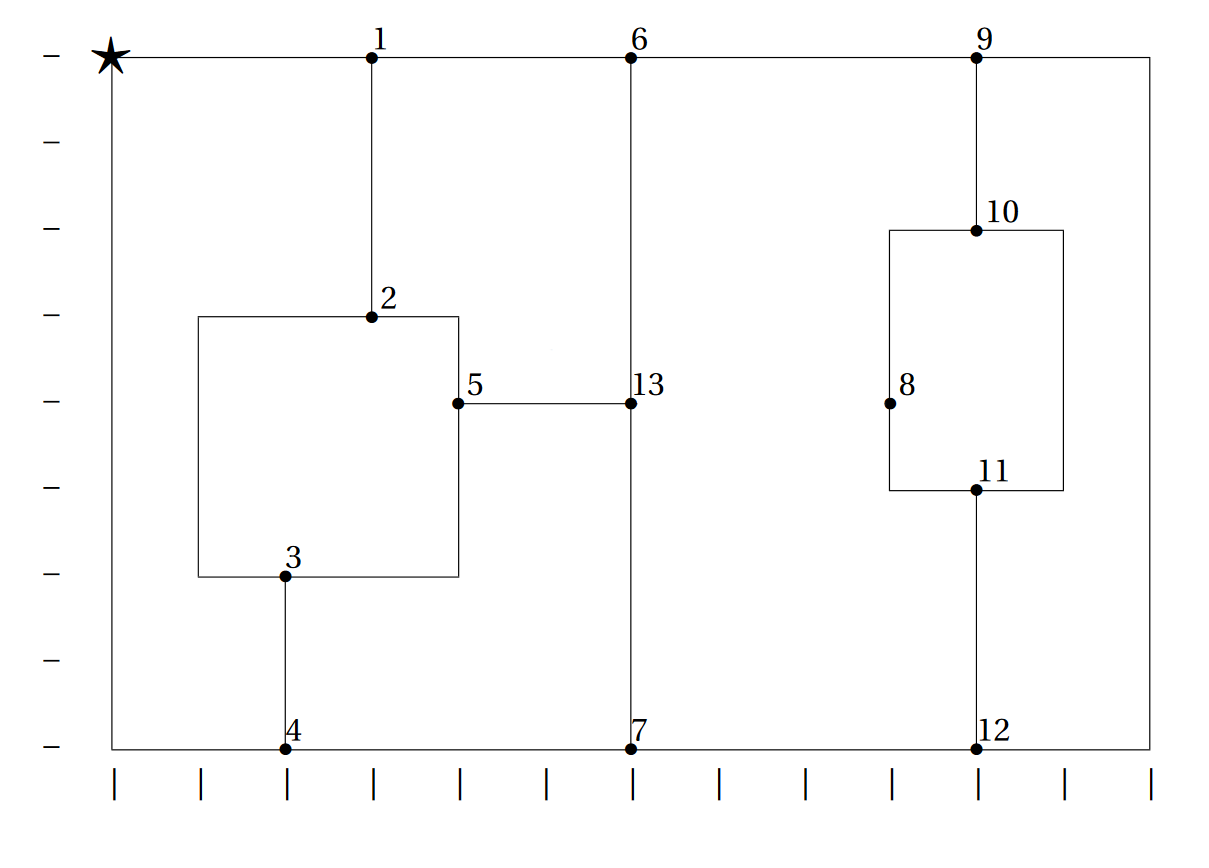
\includegraphics[width=\linewidth]{fig1.png}
    \caption{Mapa de linhas de alta tensão.}
    \label{mapa}
\end{figure}

Analisando com atenção o problema, chegamos à conclusão que o caminho que o nosso drone tem que percorrer deve ser um caminho Euleriano, ou mais especificamente um circuito Euleriano, pois deve começar e terminar o caminho no mesmo ponto. Um caminho Euleriano é um caminho de um grafo em que todas as arestas são percorridas uma única vez. Esta seria a solução ideal do nosso problema, mas, tal como diz o Teorema de Euler, apenas podemos ter um circuito Euleriano se todos os vértices do nosso grafo tiverem um grau par. Esse não é o caso no mapa que temos, logo para podermos ter um circuito Euleriano teremos que adicionar arestas ao mapa.

Chegamos desta forma ao nosso problema de otimização: \emph{que arestas é que temos que adicionar ao nosso mapa para que o caminho percorrido pelo drone seja Euleriano, e desta forma minimizar a distância total que percorre.}

Esta distância que temos de minimizar é o comprimento das arestas que iremos adicionar ao mapa, podemos ignorar o comprimento das linhas de alta tensão, pois o drone terá obrigatoriamente que as percorrer, logo esse valor será sempre constante.

Tal como referimos há pouco, para podemos ter um circuito Euleriano, todos os vértices do mapa devem ter grau par. Deste modo, as arestas a adicionar devem ligar pares de vértices de grau ímpar. Na figura seguinte assinalámos todos os vértices do nosso mapa com grau ímpar, e que teremos que ligar com arestas, que podem incidir em linhas de alta tensão ou não.

\begin{figure}[h]
    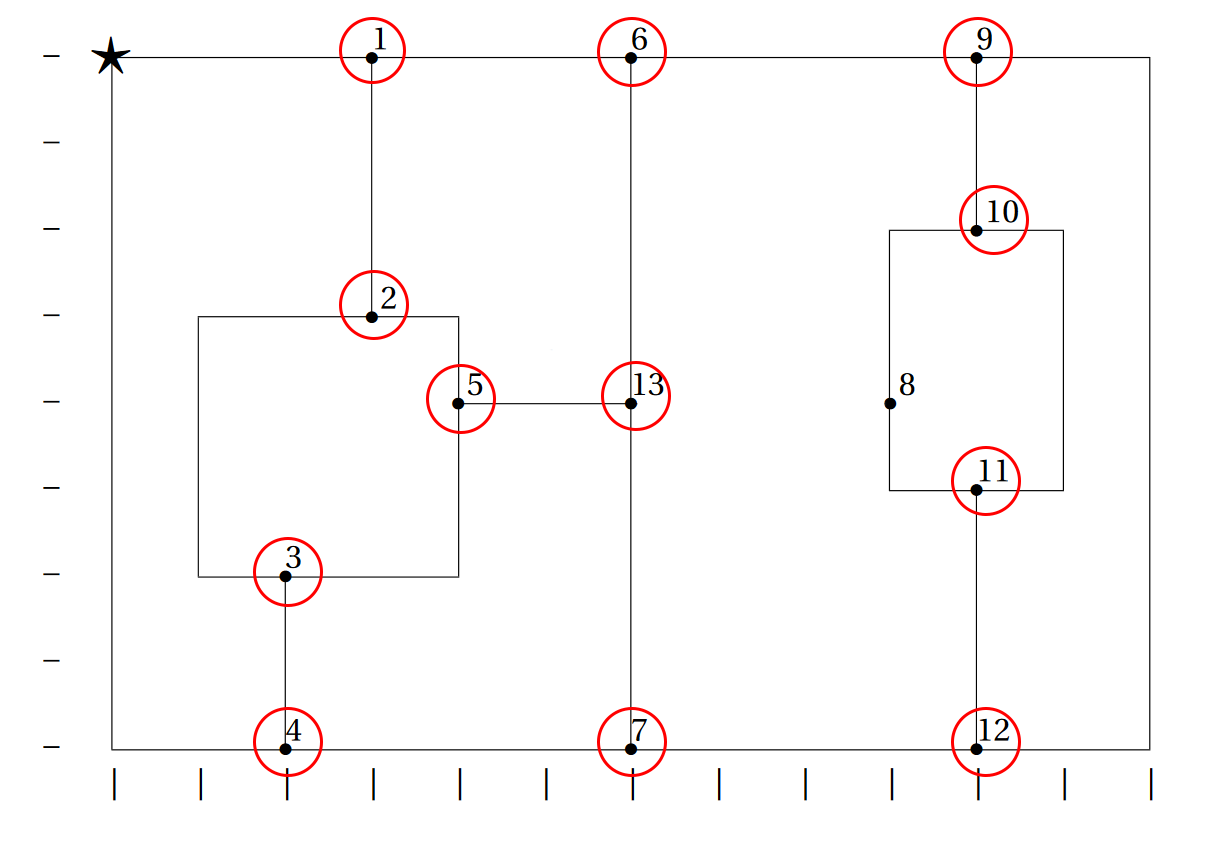
\includegraphics[width=\linewidth]{fig2.png}
    \caption{Vértices de grau ímpar.}
    \label{verticesimpares}
\end{figure}

\section{Modelo}

NOTA: Decidimos usar o sistema hexadecimal (base 16) para representar os vértices nas variáveis de decisão, dado que temos mais que 10 e menos que 16 vértices, e assim podemos representar todos os vértices com apenas um dígito. Deste modo, os vértices 'a' a 'd' correspondem aos vértices '10' a '13'.

\subsection{Variáveis de decisão}

\(x_{ij}\): existe ou não uma aresta a unir os vértices \emph{i} e \emph{j}\\
\(x_{ij} \in \{ 0,1 \}; i, j \in \{ 1, d \}; i \neq j \)

\subsection{Parâmetros}

Comprimento da aresta que une \emph{i} e \emph{j}.

\subsection{Função objetivo}

\dots

\subsection{Restrições}

\dots

\section{Análise do modelo}

\dots


\end{document}